\section{Dual Multiscale Camera (DMC)}\label{sec:dmc}
Aurora simultaneously evolves on $B_\perp$ scale widths from micro $\sim \unit[10]{m}$ to global $\sim \unit[1000]{km}$.
Within this auroral scale width range there is a continuüm of process scales continually evolving.
Instruments such as THEMIS are designed to observe the auroral oval across the width of North America simultaneously, but at low frame rate with all-sky FOV.
The ASK instrument observes with $3^\circ$ FOV at multiple narrowband wavelengths.
A key novelty of DMC was the simultaneous bandstop prompt emission filtered observation at \unit[33]{ms} cadence at $50^\circ$ and $6^\circ$ FOVs, from a single site.

DMC was constructed in part using cameras obtained for prior experiments such as Mishap and earlier work, funded under NSF EAGER contract \#FA9550-11-1-0356.
Running \$40K each EMCCD and sCMOS cameras designed for clean lab biological operations in short bursts for fluorescence microscopy is quite different than running for 12 hour stretches each night in a shed or box.
The Mishap system \citep{plant2011} deployed in 2011 near Fairbanks, AK experienced significant difficulty with dropped frames and lost timing of frames, using the system timing diagram of Figure~\ref{fig:mishap}.
\begin{sidewaysfigure}
    \includegraphics[page=2,width=0.95\linewidth]{gfx/ProposedTimingSystem}
    \caption{Mishap timing system block diagram form 2010-2011.}\label{fig:mishap}
\end{sidewaysfigure}
Some of these issues were algorithmic, and some were due to the single-core Intel Core 2 Duo E7500 CPU used in Mishap versus the far more powerful quad-core Intel Sandy Bridge i7-2600K CPU used for DMC and the even more powerful quad-core Intel Haswell i7-4790 CPU used for HiST.
As is inherently the case, little insight is gained when comparing different CPU architectures based on clock speed, particularly with on-chip GPUs in processors as modest as the \$25 Raspberry Pi allowing full-screen HD video playback and recording.
Intel Sandy Bridge and newer CPUs made numerous architecture changes \citep{lempel2011}, of which a few are particularly important for high-speed scientific video recording and processing, including:
\begin{enumerate}
    \item elimination of Front Side Bus (bottleneck for RAM and PCI Express cards)
    \item per \#1, bringing the memory controller onto the CPU die
    \item AVX SIMD floating point math-large improvements in automatic vectorization of for loops and other parallelizable problems
\end{enumerate}
The efficiency gains for math operations common to DMC/HiST gave at least a five-fold improvement in processing time.
The same is true for the TRANSCAR energy deposition modeling discussed in section~\ref{sec:fwd}.

The DMC instrument was conceived as a dual-purpose mission:
\begin{enumerate}
    \item test imaging and processing technology essential to HiST functionality
    \item explore correlations between microscale (\unit[0.1..1]{m} width) and mesoscale $\gg \unit[1]{km}$ auroral structure on \unit[20]{ms} timescales
\end{enumerate}
More specifically, DMC mission goals included:
\begin{enumerate}
	\item Two cameras successfully run at full speed for 8 hours, with data rates approaching \unit[500]{MB/s}
	\item Two cameras frame synchronized to better than $\unit[10^{-3}]{s}$
	\item Autonomous system controlled remotely from Internet bandwidth as low as \unit[5]{kB/sec} and latencies $ > \unit[250]{ms}$, using open-source tools
	\item Timing LED device (binary counter) to verify that system doesn't drop or duplicate frames, and that two separate PCs/Cameras are synchronized to specification
	\item Fully automated scheduler (runs without human intervention till hard drives fill)
    \item Sends daily start/stop recording emails, posts logs
	\item online updates with current images posted every $N=60$ seconds
    \item Many debug/disable/error points conveniently located in code
	\item Measured CPU usage during data acquisition $< 10$\%
	\item 16-bit raw grayscale data preserved with lossless compression
	\item actual experiment configuration for each recording stored in XML headers (human-readable) detailing many pertinent camera and algorithm settings, for science and engineering analysis
	\item Programs kept simple enough for research outreach, bringing students quickly to do meaningful work on parts of the program
	\item Data headers human-readable, data format easily accessible via open-source tools.
\end{enumerate}
These mission goals were met and the robustness of the HiST system was greatly improved by having the critical concepts tested in a real field system before deploying the significantly more complicated HiST stations.

\FloatBarrier
\subsection{DMC Build and Deployment}
The benchtop setup of DMC is shown in Figure~\ref{fig:dmcbench}.
\begin{figure}\centering
	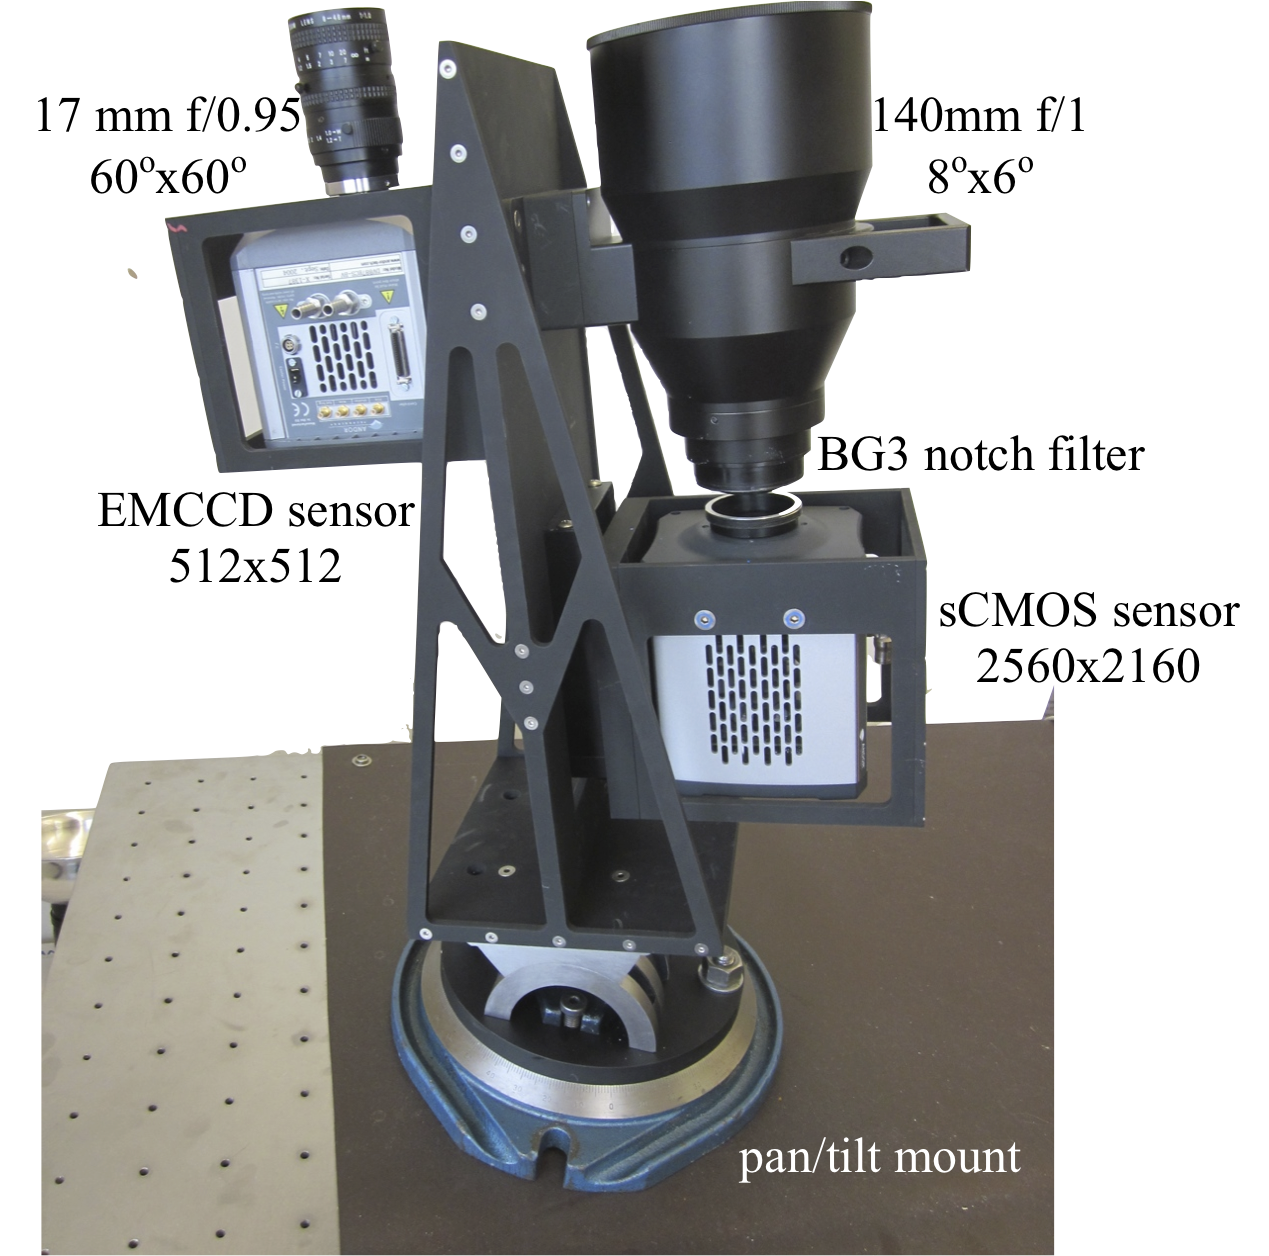
\includegraphics[width=\linewidth]{gfx/DMC_bench1}
	\caption{DMC benchtop setup. 
		At left is iXon EMCCD camera with a \unit[17]{mm} lens yielding a $50^\circ$ usable FOV. 
		At right is Neo sCMOS with 140mm lens yielding $6^\circ$ FOV. 
		Both cameras employ BG3 bandstop filters.
		The pan/tilt mount was fixed to be approximately centered on local magnetic zenith, and was constructed by Heitor Murato and Glenn Thayer of BU SIF.}
	\label{fig:dmcbench}
\end{figure}
The iXon camera at left had a usable FOV of $50^\circ \times 50^\circ$ and the Neo camera at right had a usable FOV of $6^\circ \times 8^\circ$.
Both cameras were BG3 filtered as in Figure~\ref{fig:BG3trans} to select prompt emissions as described in section~\ref{sec:physicsemissions}.
It was discovered upon deployment under the dome at Søndrestrøm that the dome was acting as a lens in the near field of the large aperture \unit[140]{mm} Neo lens.
This was confirmed by removing the dome as in Figure~\ref{fig:nodome}, which immediately gave ideal focus.
A flat glass aperture was promptly constructed and installed by Eggert Guðmundsson and crew as depicted in Figure~\ref{fig:dmcflat}.
\begin{figure}\centering
	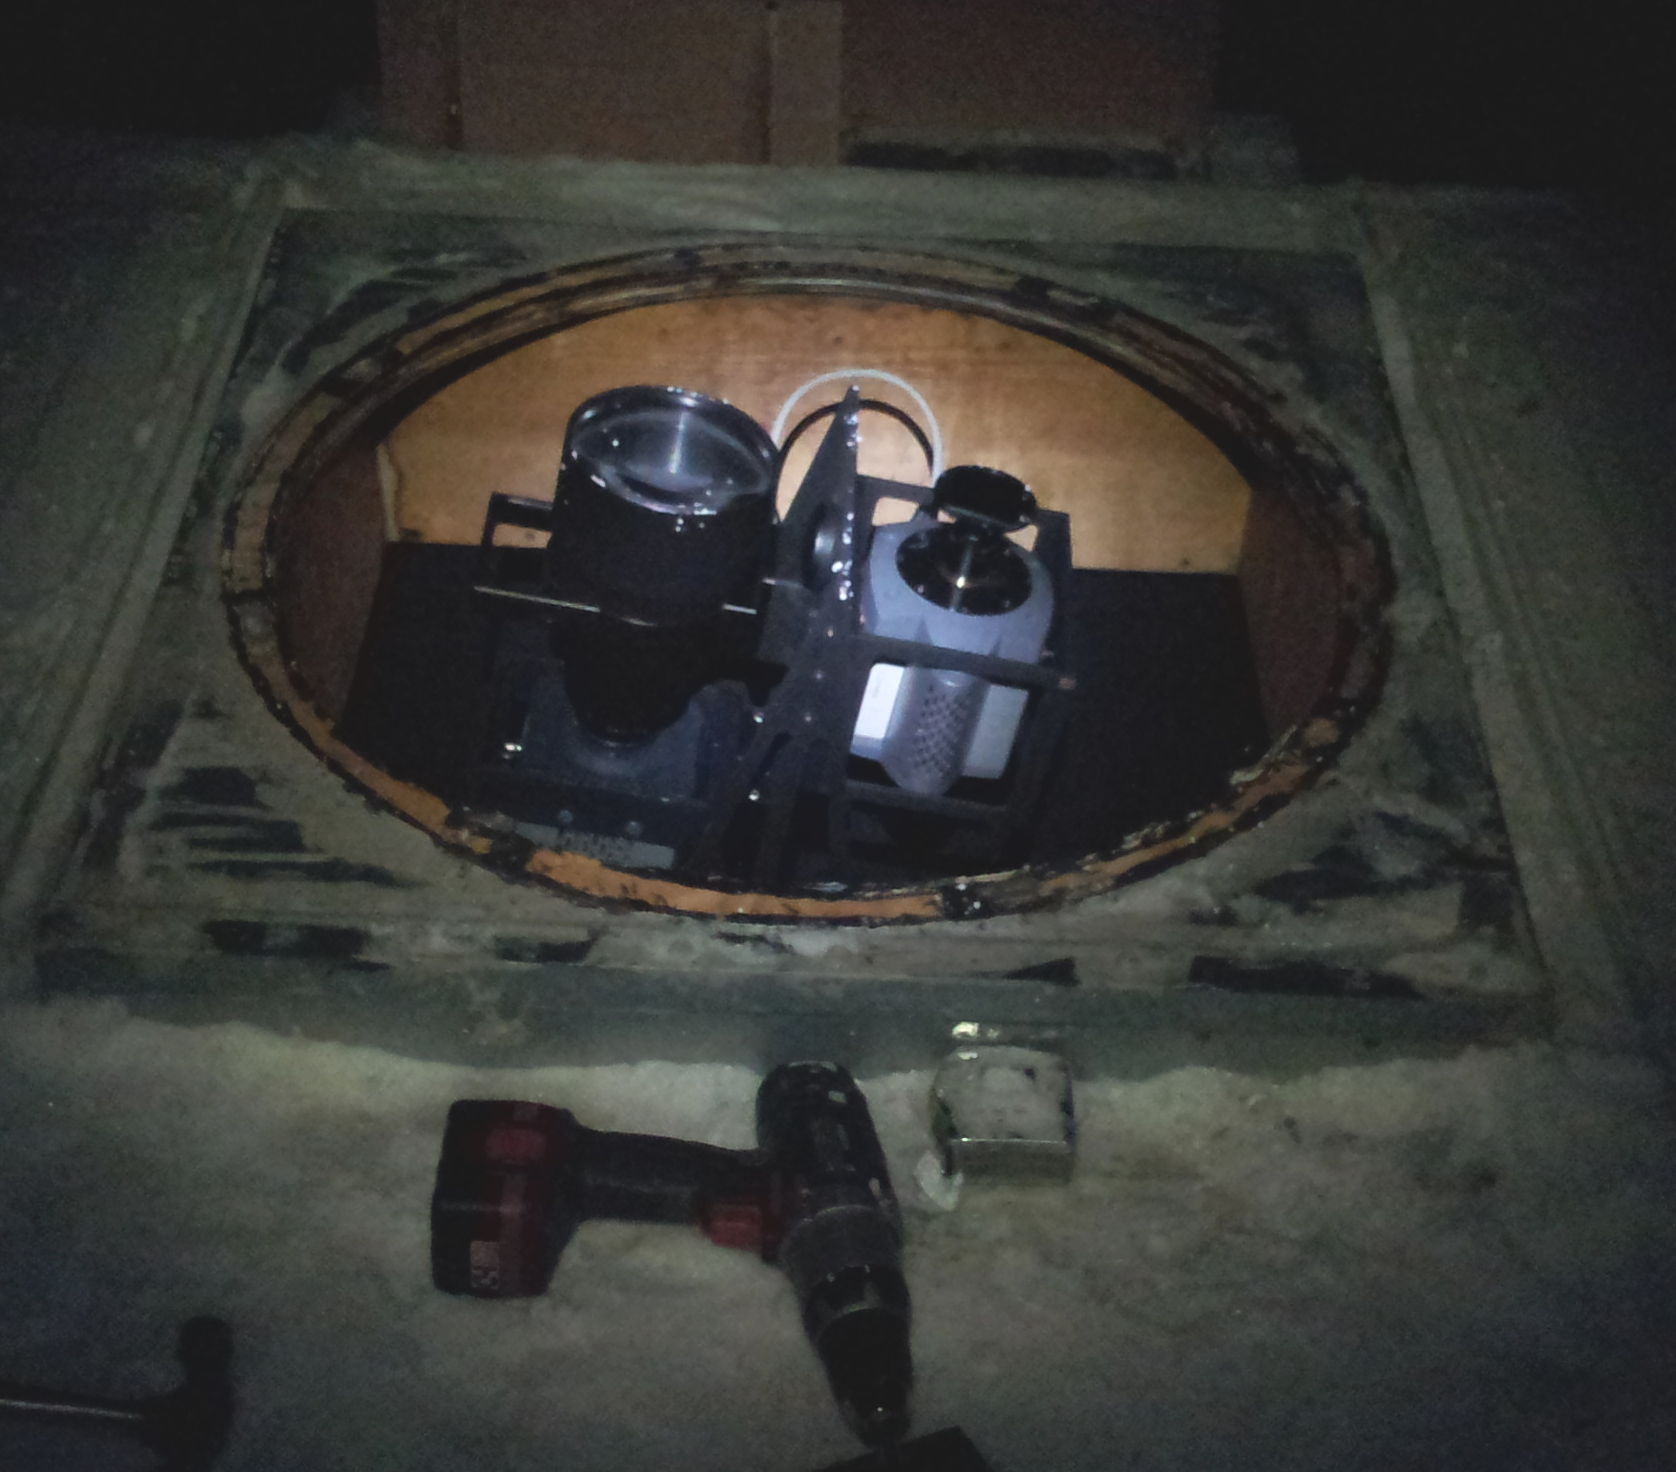
\includegraphics[width=\linewidth,trim=0 500 0 200,clip]{gfx/DMC_deployed_nodome}
	\caption{DMC installation at Søndrestrøm with dome removed for testing.}
	\label{fig:nodome}
\end{figure}
\begin{figure}\centering
	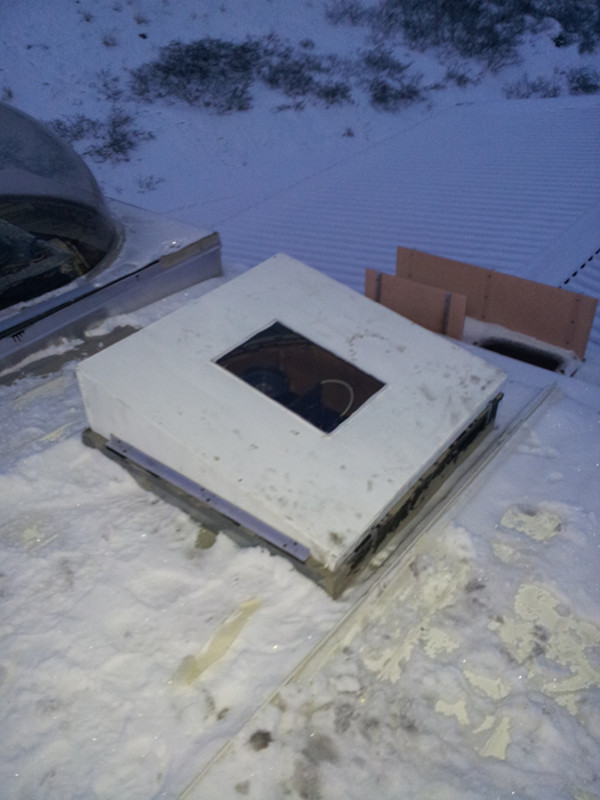
\includegraphics[width=\linewidth,trim=0 200 0 200,clip]{gfx/DMC-opening}
	\caption{DMC installation at Søndrestrøm with flat glass aperture, giving best possible focus.}
	\label{fig:dmcflat}
\end{figure}
Despite old-age failure and repair of the iXon camera and initial severe issues with the Neo camera driver, the DMC instrument was successful and has supported additional multi-instrument experiments.
DMC remains on site and ready to serve at Søndrestrøm ISR.


\FloatBarrier
\subsection{DMC Data}
DMC quickly yielded interesting data, which has been archived and will be exploited in future work.
Once DMC was working, the focus shifted to HiST build and deployment to take advantage of the same auroral season.
A sample of the novel data coming from DMC is given in Figure~\ref{fig:dmcsplit}.
\begin{figure}
	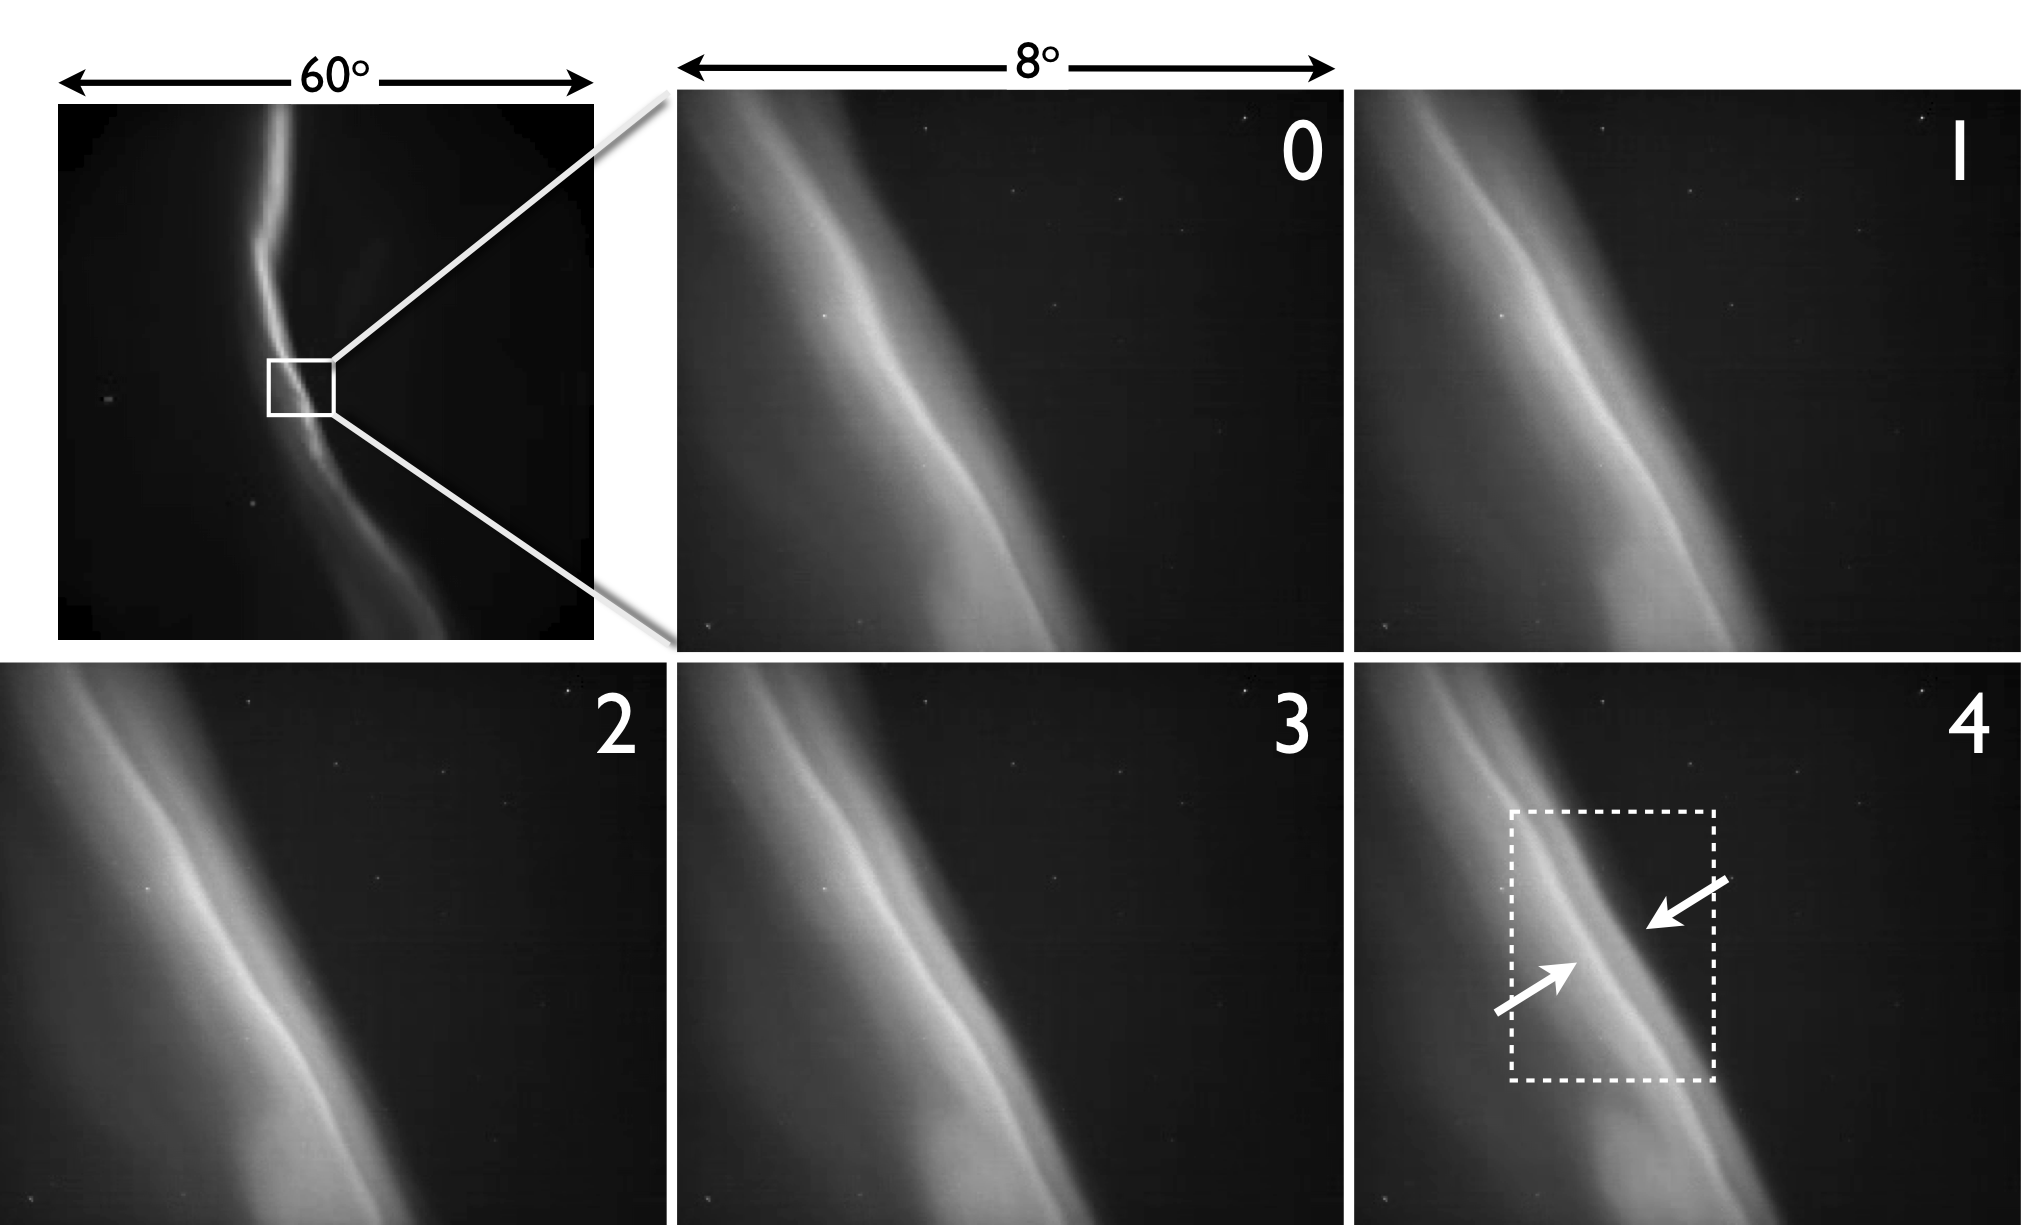
\includegraphics[width=\linewidth]{gfx/DMC_samples}
	\caption{Example of multiscale insights from DMC on 13 JAN 2013. The upper-left wide FOV images comes from the EMCCD at \unit[33]{fps}, while the \unit[50]{fps} Neo sequence in subpanels 0-4 reveals the fine scale structure invisible to the wide field camera.}
	\label{fig:dmcsplit}
\end{figure}
The splitting arc evolution of \unit[200]{m} width in Figure~\ref{fig:dmcsplit} requires tomographic analysis to quantify the Alfvén wave-driven precipitation causing the arc.
A splitting arc was observed with HiST and PFISR and is analyzed in section~\ref{sec:split}.
Another spitting auroral arc was observed with the cropped image sequence in Figure~\ref{fig:dmcsplit2}.
\begin{sidewaysfigure}
	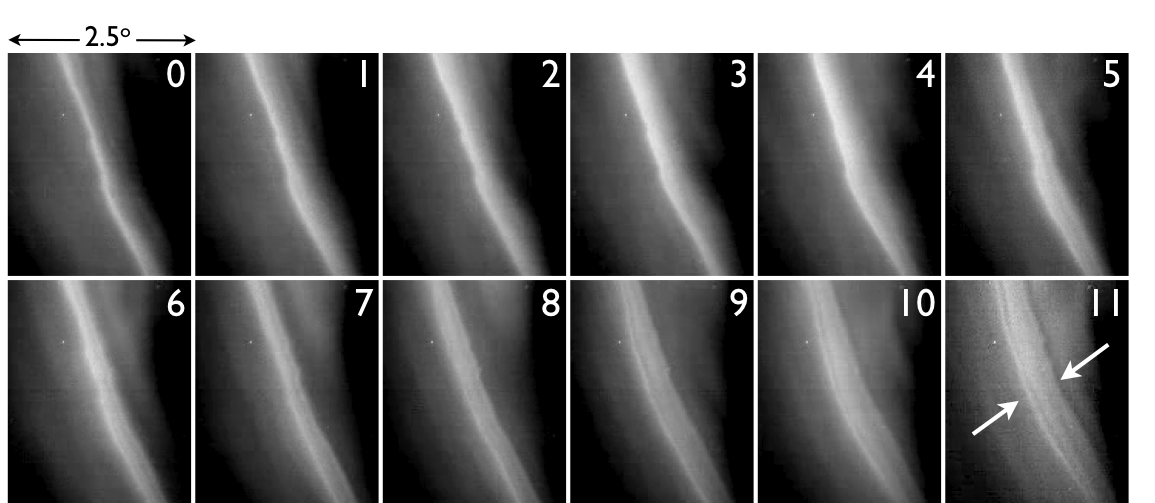
\includegraphics[width=\linewidth]{gfx/packet}
	\caption{Evolution of splitting arc as observed by Neo sCMOS narrowfield camera. The faint splitting structure would likely be washed out and smeared over by \unit[557.7]{nm} and \unit[630.0]{nm} emissions if not for the bandstop BG3 filter employed.}
	\label{fig:dmcsplit2}
\end{sidewaysfigure}
This fine structure would be completely missed in a widefield camera due to the fine sub-\unit[100]{m} structure.
Finally, a filamentary auroral arc that could come from inverted-V aurora and/or Alfvénic accelerated electrons is shown in Figure~\ref{fig:dmcfil}.
\begin{sidewaysfigure}
	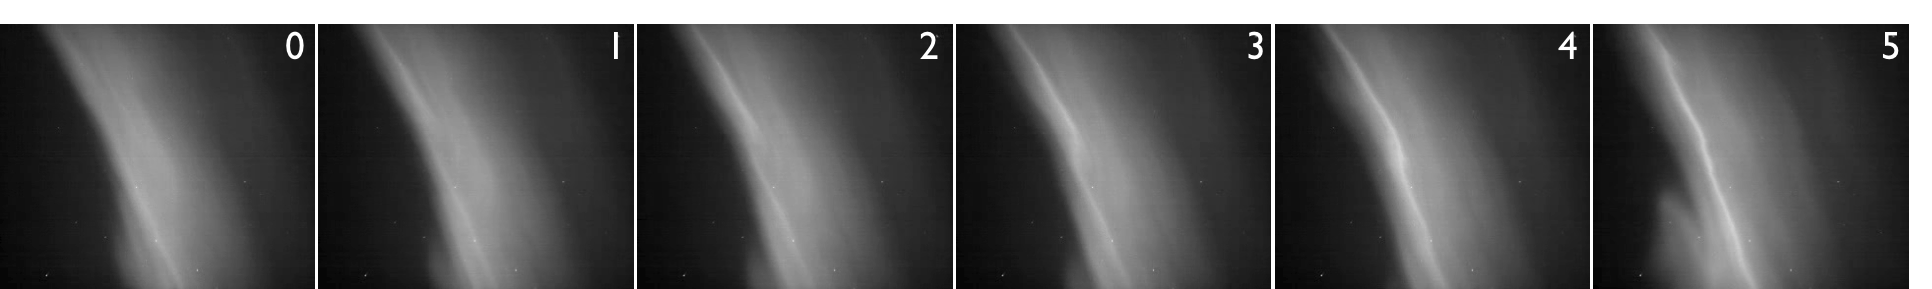
\includegraphics[width=\linewidth]{gfx/filament}
	\caption{Filamentary arc observed by DMC. Determining source acceleration would require a system like HiST to provide differential number flux estimates vs. time.}
	\label{fig:dmcfil}
\end{sidewaysfigure}
Determining source acceleration would require a system like HiST to provide differential number flux estimates vs. time.
These examples are a small taste of the data archived. 
Using the algorithms refined with HiST for joint ISR-optical analysis, future work is anticipated to analyze the single-site cameras data with Søndrestrøm ISR data.
The fast plasma line receiver estimates of electron density will be useful for recent data collected as another data fusion input \citep{vierinen2016}.

As an initial interpretation of these data, it is well established that field-aligned bursts of low energy electron precipitation occur at the edges of dynamic auroral forms. 
ISR measurements have identified anomalous ionospheric turbulence in these regions \citep{akbari2012}. 
\citet{akbari2013} revealed that this edge turbulence appears in thin layers at ranges where the ionospheric density gradients become zero (e.g., the F-region peak, and E-to-F region transition trough). 
Initial DMC observations have revealed a subtle optical signature in this region that appears as a damped outward propagating wave with wavelength $\sim \unit[300]{m}$ in Figure~\ref{fig:dmcsplit2}. Further accumulation of data will establish whether this is a consistent feature at auroral edges; and, finally, systematic comparison with space-borne and ground-based measurements will establish the electrodynamic context of these features and their consequences for communications, navigation, and high-latitude radar discrimination.

%\FloatBarrier
\subsection{Neo Burst Performance Characteristics}
Previous experiments \citep{dahlgren2013} had the operator sitting up all night waiting for aurora to press Record.
This level of human effort is not sustainable in the long term.
Obviously this method misses the build up time to interesting events, and stands a good chance of missing the desired events as well.
Nonetheless, this is how much high-speed auroral observation has taken place prior to about 2010.

For \citet{dahlgren2013} to achieve usable frame rates at full resolution, burst mode was used.
Burst mode uses the on-board camera memory in a short burst, upon which recording stops and the camera RAM is read to the PC RAM over the 3-tap Cameralink interface.
Neither binning or reducing width (width is the 2560 pixel dimension) helps improve frame rates.
Measurements were taken in Table~\ref{tab:neofullburst} at full frame.
\unit[$10^{-5}$]{s} is the minimum possible exposure time of Neo, which is much too short for auroral observations.
\unit[$10^{-3}$]{s} is roughly the minimum useful exposure time for aurora.
\unit[$10^{-2}$]{s} is about the fastest rate the companion iXon would run at. 
At full frame, the iXon can image at \unit[33]{ms} rate.
\begin{table}\centering
	\caption{Andor Neo full-frame burst imaging characteristics}\label{tab:neofullburst}
	\begin{tabular}{p{5em}p{4.5em}p{4.5em}p{5.5em}p{5em}p{5em}}
		\toprule
		Exp. Time (sec.) &  Width (pixels) & Height (pixels) &  Frames / sec &  Max \# of frames &  Max. Burst Time (sec.) \\
		\midrule
		$10^{-5}$ & 2560 & 2160 & 48.95 & 160 & 3.27 \\
		$10^{-3}$ & 2560 & 2160 & 46.68 & 160 & 3.43 \\
		$10^{-2}$ & 2560 & 2160 & 32.87 & 160 & 4.87 \\
		\bottomrule
	\end{tabular}
\end{table}
To optimize viewing area versus frame rate, the data in Table~\ref{tab:neooptburst} was collected.
Neo burst mode performance is optimized by exploiting Neo sCMOS sensor read geometry (center outward)--center on sensor.
\begin{table}\centering
	\caption{Neo burst performance with less than full-height image}\label{tab:neooptburst}
	\begin{tabular}{p{5em}p{4.5em}p{4.5em}p{5.5em}p{5em}p{5em}}
		\toprule
		Exp. Time (sec.) & Width (pixels) & Height (pixels) & Frames / sec & Max \# of frames & Max. Burst Time (sec.) \\
		\midrule
		$10^{-5}$ & 2560 & 1000 & 103.79 & 344 & 3.31\\
		$10^{-5}$ & 2560 & 512 & 197.58 & 667 & 3.38\\
		$10^{-5}$ & 2560 & 256 & 375.64 & 1315 & 3.5\\
		\midrule
		$10^{-3}$ & 2560 & 1000 & 94.12 & 344 & 3.65\\
		$10^{-3}$ & 2560 & 512 & 165.26 & 667 & 4.04\\
		$10^{-3}$ & 2560 & 256 & 273.82 & 1315 & 4.8\\
		\midrule
		$10^{-2}$ & 2560 & 1000 & 67.53 & 344 & 5.09\\
		$10^{-2}$ & 2560 & 512 & 79.87 & 667 & 8.35\\
		$10^{-2}$ & 2560 & 256 & 88.33 & 1315 & $\rightarrow\infty$\\
		\bottomrule
	\end{tabular}
\end{table}
From Table~\ref{tab:neooptburst} and the lens chosen, useful video is not obtained outside of \unit[5]{s} bursts. 
A sustainable mode of operation preserving FOV but sacrificing the excess resolution was required for the DMC mission.

%\FloatBarrier
\subsection{Neo Sustained Recording Performance Characteristics}
The Andor Neo sustained data rates are \textit{substantially} lower than burst mode rates due to the limited 3-tap Cameralink bandwidth.
The Andor Zyla 10-tap Cameralink has significantly higher frame rates than Neo with same sCMOS sensor.
Binning (creating macropixels by grouping adjacent pixels) is the key to sustained useful recording with the Andor Neo.
The maximum sustained frame rate with the Andor Neo using Solis 4.29.30012.0 is given in Table~\ref{tab:neomax}.
The Neo frame rates at 4x4 and 8x8 binning are comparable with the Andor iXon full frame rate.
\begin{table}\centering
	\caption{Neo maximum sustained frame rate with binning}\label{tab:neomax}
	\begin{tabular}{ccc}
		\toprule
		binning & width x height & frames / sec \\
		\midrule
		1x1 & 2560 x 2160 & 20 \\
		2x2 & 1280 x 1080 & 32 \\
		4x4 & 640 x 540 & 54 \\
		8x8 & 320 x 270 & 109 \\
		\bottomrule
	\end{tabular}
\end{table}


%\FloatBarrier
\subsection{Andor Neo DMC Resolution}
The Andor Neo camera has excess resolution for the planned FOV, so the Neo was typically binned 8x8.
An example of the excellent resolution of a splitting auroral arc at these Neo settings is given in Figure~\ref{fig:neosplit}.
\begin{figure}
	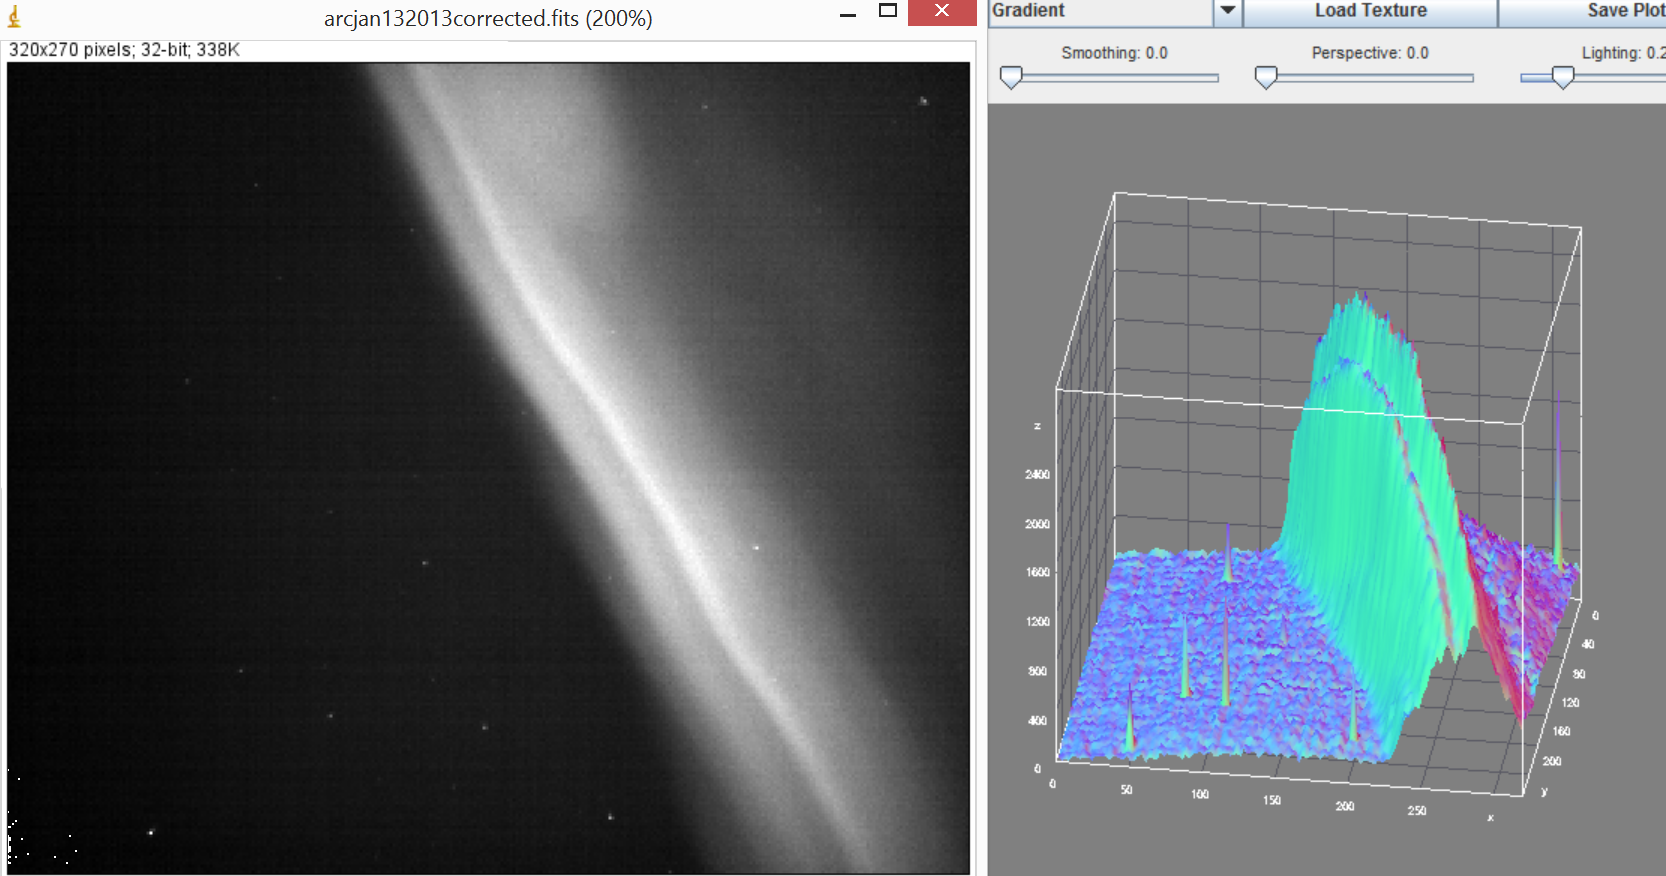
\includegraphics[trim=0 0 50 40,clip,width=\linewidth]{gfx/2013-01-13gradient}
	\caption{Splitting arc seen by DMC Neo camera, Jan 13, 2013}\label{fig:neosplit}
\end{figure}
The 3-D view of image intensity seen in the right panel of Figure~\ref{fig:neosplit} shows the fine quality of the focus and resolution with stars appearing as isolated peaks that stay nearly constant from one frame to the next.


\FloatBarrier
\subsection{Andor iXon DMC performance}
The Andor iXon 897 EMCCD (ca. 2003, serial X-1387, EEPROM ver. 6) used for DMC, like the Neo, was a camera reused from earlier projects.
As an EMCCD camera, with the iXon, objects totally invisible to eye \& Fourier analysis on Neo or Zyla can be seen in fine detail with iXon 897 under low-light conditions.
A comparison of important specification between the Neo and iXon is given in Table~\ref{tab:neoixon}.
\begin{table}\centering
	\caption{Comparison of important specification between iXon and Neo}\label{tab:neoixon}
	\begin{tabular}{rcc}
		\toprule
		Item: & iXon 897 & Neo \\
		\midrule
		Photo-electron sensitivity & $<1$ & 2.5 \\
		Pixels (w x h) & 512 x 512 & 2560 x 2160 \\
		Pixel size (microns) & 16 & 6.5 \\
		Sensor size (mm) & 8.2 x 8.2 & 16.6 x 14.0 \\
		Binning & on-chip & software \\
		Binning helps FPS? & YES & NO \\
		Reducing Width helps FPS? & NO & NO  \\
		Reducing Height helps fps, nearest: & bottom of sensor & center of sensor \\
		Minimum air cooling (deg. C) & -40 & -30 \\
		\bottomrule
	\end{tabular}
\end{table}
Images near the magnetic zenith tend to be the brightest by~\eqref{eq:bint}, so wide dynamic range is necessary. 
Because HiST and DMC work several degrees away from magnetic zenith, and faint structures embedded in bright structure is important.
Recent advances in EMCCD technology, after DMC was deployed have taken away the frame rate advantage of the sCMOS cameras for the moment.
HiST is known to have observed faint highly dynamic aurora, just above the noise floor.
These dynamic auroral forms are too faint for the Neo or Zyla sCMOS cameras to detect above the higher noise floor of the sCMOS instrument.
The higher resolution of sCMOS is useful for hyperspectral imagers like LiCHI \citep{goenka2016} that need four simultaneous images.
